\documentclass[a4paper,12pt]{report}
\usepackage{hyperref}
\usepackage{graphicx}
\usepackage{multicol}
\usepackage{color}
\usepackage{caption}
\usepackage{setspace}
\usepackage{amssymb,amsmath}     
\usepackage{tikz}
\usepackage{float}
\usetikzlibrary{decorations.pathreplacing}
%\usepackage{amsfonts,amsrefs}
\usepackage{bm}          
\usepackage{tabularx}
\usepackage{enumerate}
%\usepackage[authoryear,square,sort]{natbib}
%\usepackage[linesnumbered,ruled,vlined]{algorithm2e}
\usepackage{algorithmic}
\usepackage{lscape}
\makeatletter
\def\verbatim@font{\linespread{1}\normalfont\ttfamily}
\makeatother
\usepackage{pgfpages}

\begin{document}
%titlepage
\thispagestyle{empty}
\begin{center}
    \centering
%Thesis title
    {\uppercase{\Large \textbf{Wave Scattering by Submerged Elastic Vertical Barriers}\par}}
    \vspace{3cm}
    
    % Otago logo
    
\includegraphics[width=4cm]{logo.pdf}
    \vspace{2cm}
    
%Author's name
    {\Large {\bf Xavier Nuttall}\par}
    \vspace{2cm}
    
%Degree
    {\large A dissertation submitted in partial fulfilment of the requirements of the degree of Bachelor of Science with Honours\par}
    \vspace{1cm}
    
% Institution
    {\large Department of Mathematics and Statistics\\University of Otago
%Te Tari P\={a}ngarau me te Tatauranga, Te Whare W\={a}nanga o Ot\={a}go
\par}
    \vspace{1cm}
    
%Date
    {\large {Month, Year}}

\end{center}


\setcounter{secnumdepth}{-2}% 

\tableofcontents

\setcounter{secnumdepth}{4}% 

\chapter{Introduction}
In recent years, there has been a growing interest in coastal protection strategies due to increased coastal erosion stemming from climate change, rising sea levels. One widely adopted coastal protection method is the use of wave attenuation systems[cite...], which aim to reduce the energy of incoming waves by reflecting and dissipating it.

A significant body of research has been devoted to studying wave scattering by surface-piercing barriers[cite...], floating elastic structures[cite...], and porous vertical barriers[cite...]. However, there is little research into scattering by submerged elastic vertical barriers. This report aims to build upon the existing liturature on submerged elastic vertical barriers with a focus on ground standing barriers.

\chapter{Rigid Vertical Barrier}
\section{Mathematical Model}
\label{sec:mathModel}
We analyze the scattering of linear water waves by a submerged, bottom-standing vertical barrier located at the origin in a two-dimensional Cartesian coordinate system. The coordinate system is defined such that $x$ represents the direction of wave propagation, and $z$ denotes the vertical direction, positive upwards. The ?convention? of positive $x$ is right and negative $x$ left is adopted. We let the undisturbed water surface be at $z=0$, and the seabed is flat and horizontal at $z=-h$. A bottom-standing vertical barrier is placed at $x=0$ with the tip at $z=-d$ and the bottom at $z=-h$. 

To simplify this problem to apply classical linear water-wave thoery, assuming the wave height $\eta(x,t)$ is small relative to both the wavelength and the water depth, the free surface is approximated as $z=0$. The water is assumed to be inviscid, incompressible, and starts irrotational. The $x$ waves are assumed to be time-harmonic with angular frequency $\omega$. Thus the fluid remains irrotational. We impose a $z$-vertical no-flow condition at the seabed and a $x$-horizontal no-flow condition at the barrier. The velocity potential is defined as $\Phi(x,z,t)$, which from the time-harmonic assumption can be expressed as:

\begin{equation}
\label{eq:time-harmonic}
\Phi(x,z,t) = \text{Re}(\phi(x,z)\exp(-i\omega t)).
\end{equation}
The spacial part of the velocity potential $\phi(x,z)$ satisfies the boundary value problem (BVP):
\begin{align}
\label{eq:irrotational}
\nabla^2 \phi = 0,&  &&(x,z) \text{ not in the barrier}, \\
\label{eq:noFlowGround}
\partial_z \phi = 0,&  &&z = -h, \\
\label{eq:freeSurface}
\partial_z \phi = \frac{\omega^2}{g}\phi,&  &&z = 0, \\
\label{eq:noFlowBarrier}
\partial_x \phi= 0,&  &&x = 0, -d < z < -h.
\end{align}

\begin{figure}[h]
\centering
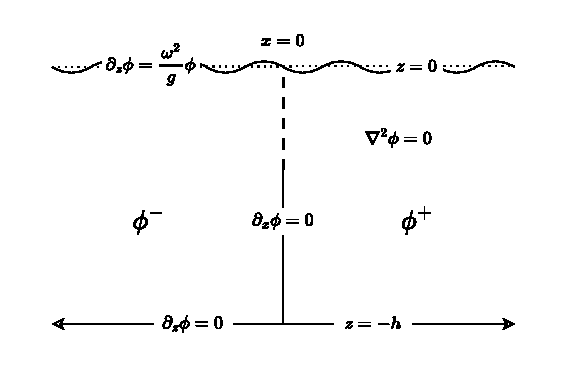
\includegraphics[width=12cm]{bvp-figure.pdf}
\caption{Diagram of the BVP}
\label{fig:bvp}
\end{figure}


Where the condition at the free surface \ref{eq:freeSurface} is derived from a simplification of the Navier-Stokes equations at the kinematic boundary condition. We then decompose the problem domain into two simple subdomains: $L = \{(x, z) \in \mathbb{R}^2 \mid x \leq 0\}$ and $R = \{(x, z) \in \mathbb{R}^2 \mid x \geq 0\}$. The governing equations \ref{eq:irrotational} to \ref{eq:noFlowBarrier} remain unchanged in each subdomain, but we impose continuity conditions, of the velocity and $x$-horizontal potential above the barrier:
\begin{align}
\label{eq:phiEquality}
\phi^- = \phi^+, &&  x=0, -d < z < -h,\\
\label{eq:phiPartialEquality}
\partial_x\phi^- = \partial_x\phi^+, &&  x=0, -d < z < -h.
\end{align}
Through separation of variables, we can express the general solution to the governing equations (\ref{eq:irrotational} to \ref{eq:noFlowBarrier}) as:
\begin{equation}
\label{eq:phiGeneralDefinition}
\phi(x,z) = \sum_{n=0}^{\infty} \big(\alpha_n\exp(ik_nx) + \beta_n\exp(-ik_nx)\big)\psi_n(z).
\end{equation}
Where $\alpha_n$ are the coefficients of the positive $x$ modes and $\beta_n$ are the coefficients of the negative $x$ modes, and 
\begin{equation}
\label{eq:psiDefinition}
    \psi_n(z) = \cosh(k_n(z+h)),
\end{equation} are the vertical eigenfunction. With the wave numbers $k_n$ above (\ref{eq:psiDefinition} and \ref{eq:phiGeneralDefinition}) being the solutions to the dispersion relation:
\begin{equation} 
\label{eq:waveNumbers}
\omega^2 = gk_n \tanh(k_nh)
\end{equation}
So letting $\phi^-$ and $\phi^+$ be the solutions in the left and right subdomains respectively, we express the general solution in each subdomain as:
\begin{align}
\label{eq:phiMinusDefinition}
\phi^-(x,z) &= \sum_{n=0}^{\infty} \big(A_n\exp(ik_nx) + B_n\exp(-ik_nx)\big)\psi_n(z),\\
\label{eq:phiPlusDefinition}
\phi^+(x,z) &= \sum_{n=0}^{\infty} \big(C_n\exp(ik_nx) + D_n\exp(-ik_nx)\big)\psi_n(z).
\end{align}
Where $A_0$ and $D_0$ are the amplitudes of the right and left propagating modes, and $B_n$ and $C_n$ are the coefficients for the reflected modes. We model only a single incident wave $A_0 = 1$, so $A_n = 0$ for all $n \geq 1$ and $D_n = 0$ for all $n$. An auxiliary function $u(z)$ is introduced above the barrier ensuring continuity between the domains [better explanation]: 
\begin{equation}
\label{eq:auxDefinition}
u(z) = \partial_x\phi^- = \partial_x\phi^+.
\end{equation}
\section{Colocation}
The goal of this method is for it to be an easy to understand baseline for which other more effective solutions and methods can be compared against.
For the colocation method, we choose a set of evenly spaced collocation points $\{z_k\}_{k=0}^{M}$ in the interval $[-h, 0]$ where $z_k = -h + kh/M$ for $k = 0, 1, \ldots, M$. We then enforce that the residual error between the left and right subdomain solutions at the collocation points is zero. We truncate the infinite series in \ref{eq:phiMinusDefinition} and \ref{eq:phiPlusDefinition} to $N$ terms so we can perform numerical calculations.
Then applying \ref{eq:phiMinusDefinition} and \ref{eq:phiPlusDefinition} into the above (\ref{eq:auxDefinition}) we have:
\begin{align}
\label{eq:auxMinusEquality}
u(z) &= \sum_{n=0}^{N} \big(A_nik_n - B_nik_n\big)\psi_n(z),\\
\label{eq:auxPlusEquality}
&= \sum_{n=0}^{N} \big(C_nik_n - D_nik_n\big)\psi_n(z).
\end{align}
Now multiplying \ref{eq:auxMinusEquality} by $\psi_m(z)$ and integrating over $z$ from $-h$ to $0$, noting that $\int_{-h}^0\psi_m(\xi)\psi_n(\xi) d\xi = 0$ for $m\neq n$ by othogonality of $\psi_n$'s we the have:
\begin{align}
\label{eq:auxMinusIntegrate}
U_m &= \int_{-h}^{0}\sum_{n=0}^{N} \big(A_nik_n - B_nik_n\big)\psi_n(\xi)\psi_m(\xi)d\xi,\nonumber\\
&= \sum_{n=0}^{N} \big(A_nik_n - B_nik_n\big)\int_{-h}^{0}\psi_n(\xi)\psi_m(\xi)d\xi,\nonumber\\
&= (A_m - B_m)P_mik_m
\end{align}
Where $U_m = \int^0_{-h}u(\xi) \psi_m(\xi) d\xi$ and $P_m = \int^0_{-h}\phi_m^2(\xi) d\xi$. Following the same process for \ref{eq:auxPlusEquality} we have:
\begin{align}
\label{eq:auxPlusIntegrate}
U_m &= (C_m - D_m)P_mik_m
\end{align}
Using \ref{eq:auxMinusIntegrate}, \ref{eq:auxPlusIntegrate}, \ref{eq:phiEquality}, \ref{eq:noFlowBarrier}, \ref{eq:auxDefinition} and $A_{n>0} = D_n = 0$, we obtain:
\begin{equation}
\label{eq:colocationSystem}
\psi_0(z) = \int_{-d}^0 K(z,\xi) u(\xi) d\xi.
\end{equation}
Where $\displaystyle K(z,\xi) = \sum_{m=0}^{N} \frac{\psi_m(z)\psi_m(\xi)}{P_mik_m}$. Now we can apply a quadrature method to obtain a system of equations for which we use to solve for $u(z_k)$, here trapezoidal quadrature is used. These collocated auxilary values can then be used to solve for $U_m$, which we can then use in \ref{eq:auxMinusIntegrate} and \ref{eq:auxPlusIntegrate} to solve for the coefficients $B_n$ and $C_n$.
\subsection{Convergence Analysis}


\section{Galerkin Method}
In this method, we approximate the solution $u(z)$ as a truncated sum of basis functions. We want these basis functions to encapsulate the singular behaviour at the tip of the barrier, caused by the change in velocity ($\partial_x \phi$) as you approach the tip from the \ref{eq:noFlowBarrier} condition. [explain the singularity as square root]. So we approximate $u(z)$ with truncation $W$ as,
\begin{equation}
\label{eq:galerkinApprox}
u(z) \approx \sum_{i=0}^{W} c_i v_i(z),
\end{equation}
where $c_i$ are the coefficients to be determined and,\\ $\displaystyle v_i(z) = ((h-d)^2-(h+z)^2)^{-1/2}T_{2i}\Big(\frac{z+h}{h-d}\Big)$, where $T_i$ are Chebyshev polynomials of the first kind. Then using this approximation in \ref{eq:colocationSystem} we have,
\begin{equation}
\label{eq:galerkinSystem}
\psi_0(z) = \int_{-d}^0 K(z,\xi) \sum_{i=0}^{W} c_i v_i(\xi) d\xi.
\end{equation}

Multiplying both sides by $v_m(z)$ and integrating over $z$ from $-d$ to $0$,
\begin{align}
\label{eq:galerkinIntegrate}
V_{0,m} &= \int_{-d}^0 \int_{-d}^0 K(z,\xi) \sum_{j=0}^{W} c_j v_j(\xi)  d\xi v_m(z) dz\nonumber\\
&= \sum_{j=0}^{W} c_j \int_{-d}^0 \int_{-d}^0 K(z,\xi) v_j(\xi)  d\xi v_m(z) dz\nonumber\\
&= \sum_{j=0}^{W} c_j \int_{-d}^0 \int_{-d}^0 \sum^N_{n=0} (ik_n P_n)^{-1} \phi_n(z)\phi_n(\xi) v_j(\xi) d\xi v_m(z) dz\nonumber\\
&= \sum_{j=0}^{W} c_j \sum^N_{n=0} (ik_n P_n)^{-1} \int_{-d}^0  \phi_n(\xi) v_j(\xi) d\xi \int_{-d}^0\phi_n(z) v_m(z) dz \nonumber\\
&= \sum_{j=0}^{W} c_j \sum^N_{n=0} (ik_n P_n)^{-1}  V_{n,j} V_{n,m}.
\end{align}
Where $V_{k,j} = \int_{-d}^0 \phi_k(z) v_j(z) dz$. We can then solve this system of equations for the coefficients $c_j$. Follwoing this we obtain an approximation of $u(z)$ to solve for the coefficients $B_n$ and $C_n$ in \ref{eq:auxMinusIntegrate} and \ref{eq:auxPlusIntegrate}, using the approximation,
\begin{equation}
\label{eq:galerkinApproxU}
U_m = \int_{-h}^{0} u(\xi) \psi_m(\xi) d\xi \approx \sum_{j=0}^{W} c_j V_{m,j},
\end{equation}
and the closed form solution \cite{bateman1954} to the $V_{m,j}$ integrals,
\begin{equation}
\label{eq:VIntegral}
V_{m,j} = \int_{-d}^{0} \phi_m(z) v_j(z) dz = (-1)^j \frac{\pi}{2} J_{2j}(ik_m(h-d)).
\end{equation}

\subsection{Convergence}
         
%\clearpage
\addcontentsline{toc}{chapter}{Bibliography}
\bibliographystyle{amsplain}
\bibliography{HonsRefs}

\newpage
\appendix


\end{document}
